\documentclass[mathserif]{beamer}
%
% Choose how your presentation looks.
%
% For more themes, color themes and font themes, see:
% http://deic.uab.es/~iblanes/beamer_gallery/index_by_theme.html
%

\mode<presentation>
{
  \usetheme{default}      % or try Darmstadt, Madrid, Warsaw, ...
  \usecolortheme{default} % or try albatross, beaver, crane, ...
  \usefonttheme{default}  % or try serif, structurebold, ...
  \setbeamertemplate{navigation symbols}{}
  \setbeamertemplate{caption}[numbered]
}

\usepackage[english]{babel}
\usepackage[utf8x]{inputenc}
\usepackage{multirow}
\usepackage{array, booktabs}
\usepackage{threeparttable}
\usepackage{dcolumn}

\usepackage{subcaption}
\captionsetup{compatibility=false}

\linespread{1.1}

\title[ConvNet for Image Classification]{ConvNet for Image Classification\\in the Study of Plankton Recognition}
\author{Xihuan Zeng, Rihan Chen, Jingxiang Li (G19)}
\institute{School of Statistics, UMN}
\date

\begin{document}

\begin{frame}
  \titlepage
\end{frame}

% Uncomment these lines for an automatically generated outline.
%\begin{frame}{Outline}
%  \tableofcontents
%\end{frame}

\begin{frame}{Problem Statement}
\begin{block}{Analysis Goal}
\begin{itemize}
  \item Classify ocean planktons given their images
  \item Input: 30,000 Images, each contains a single organism
  \item Output: 121 Labels of the plankton
\end{itemize}
\end{block}

\begin{block}{Two Stages}
\begin{itemize}
  \item Pilot Study: 7,000 images with 8 labels
  \item Complete Study: 30,000 images with 121 different labels
\end{itemize}
\end{block}


\end{frame}

\begin{frame}{Dataset}
\vspace{-1cm}
\begin{table}[ht!]
\centering
\caption{Sample from Dataset, Part 1}
\begin{tabular}{m{3pt} m{130pt} | m{120pt}}
\toprule
1 & acantharia\_protist & 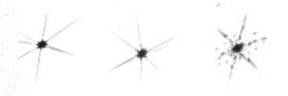
\includegraphics[scale=0.4]{./fig/acantharia_protist.png}\\
2 & appendicularian\_s\_shape & 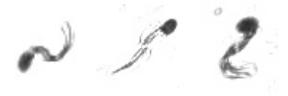
\includegraphics[scale=0.4]{./fig/appendicularian_s_shape.png}\\
4 & chaetognath\_non\_sagitta & 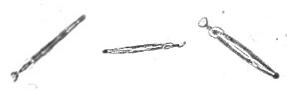
\includegraphics[scale=0.4]{./fig/chaetognath_non_sagitta.png}\\
4 & copepod\_calanoid & 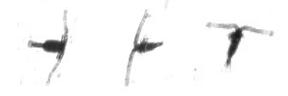
\includegraphics[scale=0.4]{./fig/copepod_calanoid.png}\\
% copepod\_cyclopoid\_oithona & 
\includegraphics[scale=0.2]{./fig/copepod_cyclopoid_oithona.png}\\
% trichodesmium\_bowtie & 
\includegraphics[scale=0.2]{./fig/trichodesmium_bowtie.png}\\
% trichodesmium\_puff & 
\includegraphics[scale=0.2]{./fig/trichodesmium_puff.png}\\
% trichodesmium\_tuft & 
\includegraphics[scale=0.2]{./fig/trichodesmium_tuft.png}\\
\bottomrule
\end{tabular}
\end{table}
\end{frame}

\begin{frame}{Dataset for Pilot Study}
\vspace{-1cm}
\begin{table}[ht!]
\centering
\caption{Sample from Dataset, Part 2}
\begin{tabular}{m{3pt} m{130pt} | m{120pt}}
\toprule
% acantharia\_protist & 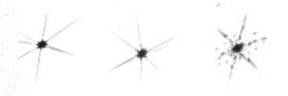
\includegraphics[scale=0.4]{./fig/acantharia_protist.png}\\
% appendicularian\_s\_shape & 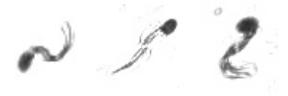
\includegraphics[scale=0.4]{./fig/appendicularian_s_shape.png}\\
% chaetognath\_non\_sagitta & 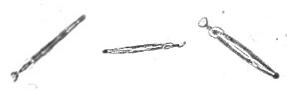
\includegraphics[scale=0.4]{./fig/chaetognath_non_sagitta.png}\\
% copepod\_calanoid & 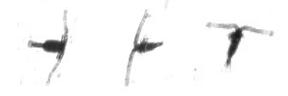
\includegraphics[scale=0.4]{./fig/copepod_calanoid.png}\\
5 & copepod\_cyclopoid\_oithona & 
\includegraphics[scale=0.4]{./fig/copepod_cyclopoid_oithona.png}\\
6 & trichodesmium\_bowtie & 
\includegraphics[scale=0.4]{./fig/trichodesmium_bowtie.png}\\
7 & trichodesmium\_puff & 
\includegraphics[scale=0.4]{./fig/trichodesmium_puff.png}\\
8 & trichodesmium\_tuft & 
\includegraphics[scale=0.4]{./fig/trichodesmium_tuft.png}\\
\bottomrule
\end{tabular}
\end{table}
\end{frame}

\begin{frame}{Data Augmentation}
\begin{columns}[t]

\column{.25\textwidth}
\begin{block}{Transformation}
\begin{itemize}
  \item Flip
  \item Rotation
  \item Rescaling
  \item Translation
\end{itemize}
\end{block}

\column{.75\textwidth}
\begin{figure}[ht!]
\centering
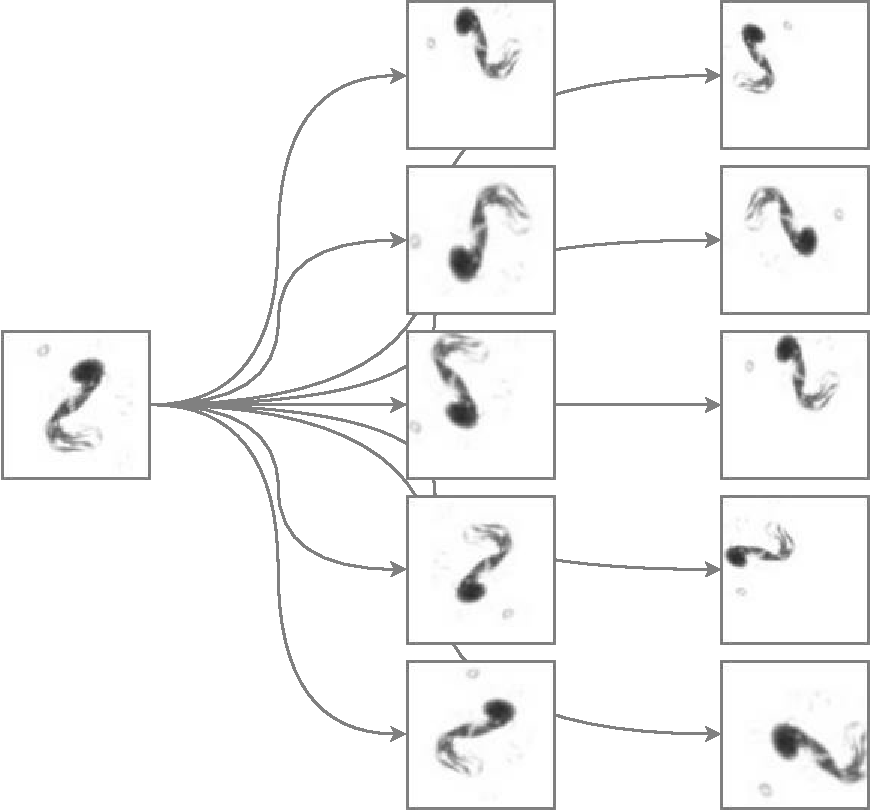
\includegraphics[width=.7\linewidth]{fig/CSci-5525-data-augmentation-crop.pdf}
\caption{Original (Left) v.s. Augmented (Right)}
\end{figure}

\end{columns}
\end{frame}

\begin{frame}{Selected Models}
\begin{block}{Deep Learning}
\begin{itemize}
\item Convolutional Neural Network (\texttt{Keras})
\end{itemize}
\end{block}

\begin{block}{Ensemble Methods}
\begin{itemize}
  \item Random Forest (\texttt{scikit-learn})
  \item Gradient Boost (\texttt{dmlc-XGBoost})
\end{itemize}
\end{block}
\end{frame}

\begin{frame}{Prediction Accuracy}
\begin{block}{Pilot Study (8 Classes)}
\begin{itemize}
\item ConvNet: $\color{red}{\mathbf{0.9365}}$
\item Gradient Boost: $0.8464$
\item Random Forest: $0.8546$
\end{itemize}
\end{block}

\begin{block}{Complete Study (121 Classes)}
\begin{itemize}
\item ConvNet: $\color{red}{\mathbf{0.674}}$
\end{itemize}
\end{block}
\end{frame}

%----------------------------------------------

\begin{frame}{ConvNet Structure}
\begin{block}{Pilot Study (8 Classes)}
\begin{itemize}
\item Modify on the ConvNet structure for \textit{cifar10} data set.
\item Relatively simple structure in terms of \textbf{depth} in case of \textit{over-fitting}.
\item 4 Convolution Layers, 2 Max Pooling Layers and 2 Fully Connected Layers.
\end{itemize}
\end{block}
\end{frame}

\begin{frame}{ConvNet Structure}
\vspace{-20pt}
\begin{table}[ht]
\centering
\footnotesize
\rmfamily
\caption{Structure of ConvNet for Pilot Study}
\begin{tabular}{lll}
\toprule
Layer & Size & Output \\
\midrule
input & & (32, 1, 32, 32) \\
augmentation & & (32, 1, 32, 32) \\
convolution & 32 $3\times3$ kernels & (32, 32, 32, 32) \\
convolution & 32 $3\times3$ kernels & (32, 32, 32, 32) \\
max-pooling & $2 \times 2$, stride 2 & (32, 32, 16, 16) \\
dropout & $p = 0.25$ & (32, 32, 16, 16) \\
convolution & 64 $3\times3$ kernels & (32, 64, 16, 16) \\
convolution & 64 $3\times3$ kernels & (32, 64, 16, 16) \\
max-pooling & $2 \times 2$, stride 2 & (32, 64, 8, 8) \\
dropout & $p = 0.25$ & (32, 64, 8, 8) \\
fully connected & 512 hidden units & (32, 512)\\
dropout & $p = 0.5$ & (32, 512) \\
fully connected & 8 way soft-max & (32, 8)\\
\bottomrule
\end{tabular}
\end{table}
\end{frame}


\begin{frame}{Real-time Data Augmentation}
Randomly modify the images during the process of optimization.

\begin{block}{Advantages}
\begin{itemize}
\item Greatly save the space for data storage: only the original data need to be kept.
\item The amount of data augmentation is simply decided by how many epochs we run.
\end{itemize}
\end{block}
\begin{block}{Price to Pay}
\begin{itemize}
\item Slow optimization compared with off-line data augmentation.
\end{itemize}
\end{block}
\end{frame}

\begin{frame}{ConvNet Structure}
\vspace{-10pt}
\begin{block}{Complete Study (121 Classes)}
\begin{itemize}
\item Modify on the ConvNet structure for \textit{cifar100} data set.
\item Enlarge the image dimension for building more complicated model.
\item Relatively complicated structure in terms of \textbf{depth}.
\item 10 Convolution Layers, 4 Max Pooling Layers and 3 Fully Connected Layers.
\end{itemize}
\end{block}
\end{frame}

%----------------------------------------------

\begin{frame}{Symbolic vs Imperative Programs}

\begin{figure}
\graphicspath{./}
\begin{subfigure}{.3\textwidth}
\centering
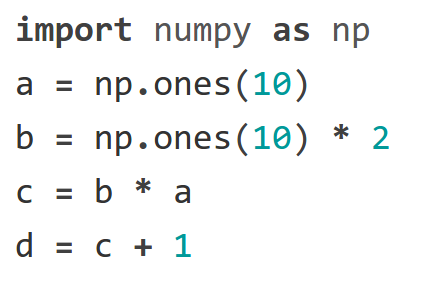
\includegraphics[width=1.1\linewidth]{fig/Imperative.png}
\end{subfigure}%
\begin{subfigure}{.65\textwidth}
\centering
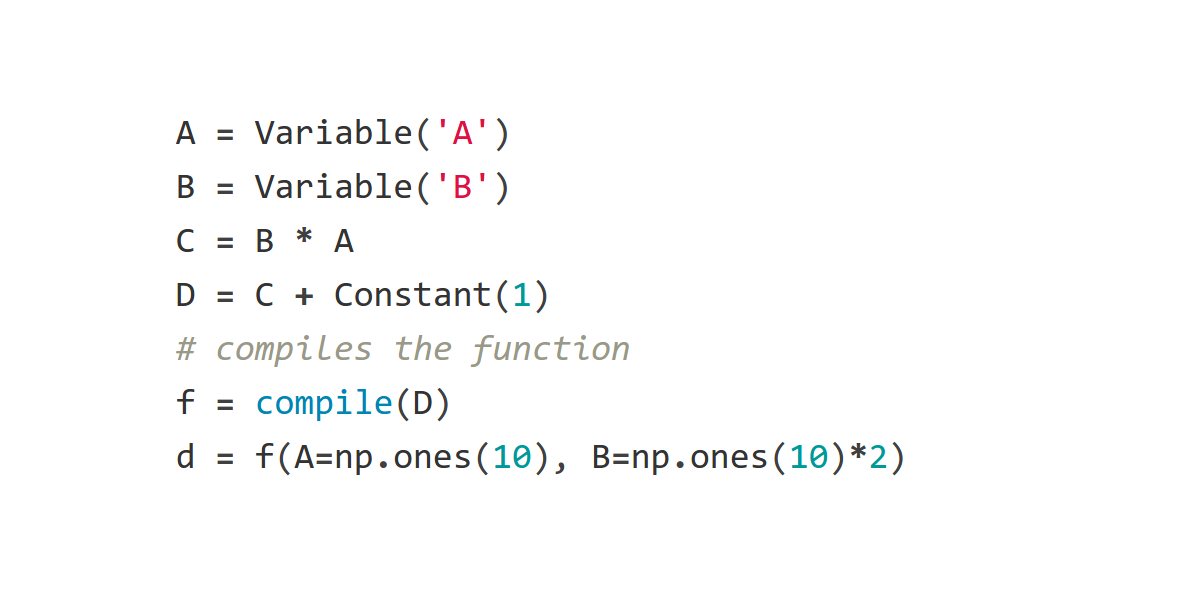
\includegraphics[width=1.4\linewidth]{fig/Symbolic.png}
\end{subfigure}
\caption{Imperative (Left) v.s. Symbolic (Right)}
\end{figure}

\end{frame}

\begin{frame}{Symbolic vs Imperative Programs}
\begin{figure}
\graphicspath{./}
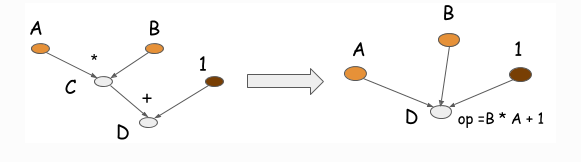
\includegraphics[width=.9\linewidth]{fig/symbolic2.png}
\caption{Graph Optimization}
\end{figure}
\end{frame}

\begin{frame}{Symbolic vs Imperative Programs}
\begin{block}{Imperative style deep learning libraries}
\begin{itemize}
\item Torch, Chainer and Minerva
\item Advantage is flexibility and easier to use native language features and inject them into computation flow.
\end{itemize}
\end{block}

\begin{block}{Symbolic style deep learning libraries}
\begin{itemize}
\item Theano, CGT and Tensorflow
\item Advantage is efficiency and space-saving
\end{itemize}
\end{block}
\end{frame}

\begin{frame}{Modern GPU and CUDA}
\begin{itemize}
\item Modern GPUs are very efficient at manipulating computer graphics and image processing, and their highly parallel structure makes them more effective than general-purpose CPUs for algorithms where the processing of large blocks of visual data is done in parallel.
\item CUDA is a parallel computing platform created by NVIDIA. The CUDA platform is designed to work with programming languages such as C, C++ and Fortran
\end{itemize}
\end{frame}

\begin{frame}{Reference}
\begin{itemize}
\item Challenge Home Page: https://www.kaggle.com/c/datasciencebowl
\item Karas: http://keras.io/
\item Symbolic Program: https://mxnet.readthedocs.org/en/latest/program\_model.html
\item CUDA: https://en.wikipedia.org/wiki/CUDA
\end{itemize}
\end{frame}
\end{document}
